\documentclass[a4paper, 11pt, normalem]{report}

\usepackage{../../../LaTeX-Templates/Notes}
\usepackage{subfiles}
\usepackage{tensor}

\usetikzlibrary{decorations.pathmorphing}
\usetikzlibrary{decorations.pathreplacing}
\usetikzlibrary{arrows.meta}
\tikzset{snake it/.style={decorate,decoration=snake}}

\def\imagebox#1#2{\vtop to #1{\null\hbox{#2}\vfill}}

\newcommand\hphi{\hat{\phi}}
\newcommand\hpi{\hat{\pi}}
\newcommand\hpsi{\hat{\psi}}
\newcommand\vy{\unl{y}}

\graphicspath{{diagrams/}}

\rhead{\hyperlink{page.1}{Contents}}

\begin{document}
\begin{titlepage}
    \newcommand{\HRule}{\rule{\linewidth}{0.5mm}}
    \center
    {
\includegraphics[scale=0.5]{../../logo0.png}\hfill{\Large\bfseries Michaelmas 2019}}\\[2.5cm]
    {\LARGE\bfseries Particle Theory}\\[1.5cm]
    \HRule \\[0.7cm]
    {\huge\bfseries Relativistic Quantum Mechanics}\\[0.4cm]
    \HRule \\[1.5cm]

    \begin{minipage}{0.4\textwidth}
        \begin{flushleft} \large
            \emph{Author:} \\ Matthew Rossetter
        \end{flushleft}
    \end{minipage}~
    \begin{minipage}{0.4\textwidth}
        \begin{flushright} \large
            \emph{Lecturer:} \\ Prof. Frank Krauss
        \end{flushright}
    \end{minipage}\\[2cm]
    \vfill
    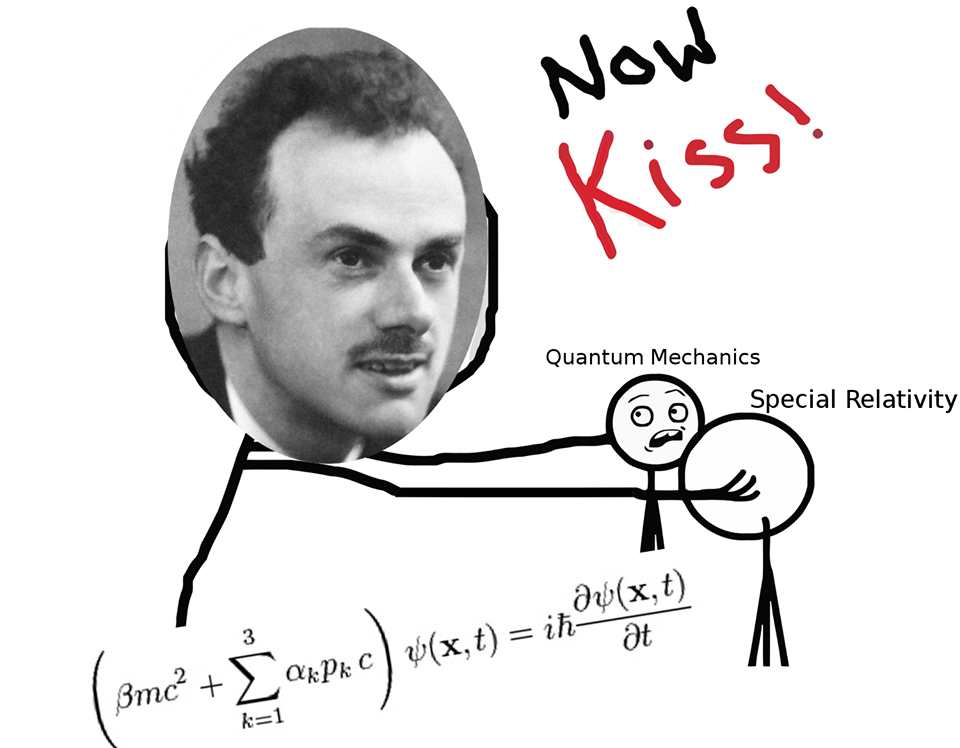
\includegraphics[width=0.8\textwidth]{rqm.png}\\[1cm]
    \vfill
\end{titlepage}
\tableofcontents

\chapter{Recapitulation of Important Ingredients}

\section{Natural Units}
\vspace{-20pt}
\begin{align}
    \hbar &= c = 1 \\
    \text{energy} &= \frac{1}{\text{length}} \\
    \hbar c &= 200\,\text{MeV}\cdot\text{fm} \\
    \text{energy} &= \text{momentum}~ (c = 3\times10^8\;\text{ms}^{-1} = 3\times10^{23}\;\text{fm s}^{-1})
\end{align}

\section{Four Vectors}
\vspace{-20pt}
\begin{align}
    p^{\mu=\{0,\dots,3\}} &= (E,\unl{p}), \\
    p^\mu p_\mu &= E^2 - \unl{p}^2 = E^2 - p_ip_i \\
    g^{\mu\nu} &= \begin{pmatrix} 1 & 0 & 0 & 0 \\ 0 & -1 & 0 & 0 \\ 0 & 0 & -1 & 0 \\ 0 & 0 & 0 & -1 \end{pmatrix} = g_{\mu\nu}, \quad
    g^\mu_\nu = I \\
    \frac{\p}{\p x^\mu} &= \p_\mu,\quad
    \frac{\p}{\p x^\mu} (x\cdot p) = p_\mu \\
    \frac{\p}{\p x_\mu} &= \p^\mu,\quad
    \frac{\p}{\p x_\mu} (x\cdot p) = p^\mu
\end{align}

Kronecker delta:
\begin{align}
    \delta_{ij} = \delta^{ij} &= \begin{cases} 1 & i=j \\ 0 & \text{otherwise} \end{cases}
\end{align}
Levi-Civita tensor:
\begin{equation}
    \e_{ijk} = \e^{ijk} = \begin{cases} 1 & \{ijk\} \text{ cyclical perm of 123} \\ -1 & \{ijk\} \text{ anti-cyclical perm} \\ 0 & \text{otherwise} \end{cases}
\end{equation}
Anti-symmetric tensor:
\begin{equation}
    \e_{\mu\nu\rho\sigma} = \e^{\mu\nu\rho\sigma} = \begin{cases} 1 & \{\mu\nu\rho\sigma\} \text{ cyclical perm of 0123} \\ -1 & \{\mu\nu\rho\sigma\} \text{ anti-cyclical perm} \\ 0 & \text{otherwise} \end{cases}
\end{equation}

\section{Lorentz Transformation}
Boosts and rotations:
\begin{equation}
    x'^\mu = \tensor{\Lambda}{^\mu_\nu} x^\nu
\end{equation}
Lorentz boost along z-axis:
\begin{equation}
    \tensor{\Lambda}{^\mu_\nu} = \begin{pmatrix} \cosh\nu & 0 & 0 & -\sinh\nu \\ 0 & 1 & 0 & 0 \\ 0 & 0 & 1 & 0 \\ -\sinh\nu & 0 & 0 & \cosh\nu \end{pmatrix}
\end{equation}
where rapidity
\begin{equation}
    \cosh\nu = \gamma - \frac{1}{\sqrt{1-\nu^2}}
\end{equation}

\section{Lagrange formalism}
\begin{align}
    L\left(q(t),\dot{q}(t)\right) &= T - V \\
    S(t,t_0) &= \int_{t_0}^t L\; dt'
\end{align}
Minimise action, $S$, leads to Euler-Lagrange equations of motion:
\begin{align}
    \frac{d}{dt} \frac{\p L}{\p\dot{q}} - \frac{\p L}{\p q} = 0
\end{align}
Introduce Hamilton function:
\begin{align}
    H(p,q) &= \dot{q}\frac{\p L}{\p \dot{q}} - L = T+V,~ \dot{q} \to p = \frac{\p L}{\p \dot{q}} \\
    \dot{q} &= \frac{\p H}{\p p},~ \dot{p} = -\frac{\p H}{\p q}
\end{align}

\section{Harmonic Oscillator, 1st quantisation}
\begin{align}
    \hat{H} &= \frac{\hat{p}^2}{2m} + \frac{m\om^2}{2}\hat{x}^2 \\
    [\hat{x},\hat{p}] &= i = \hat{x}\hat{p} - \hat{p}\hat{x}
\end{align}
Introducing the annihilation and creation operators:
\begin{align}
    \ha &= \frac{1}{\sqrt{2}}\left(\sqrt{\om}\hx + \frac{i}{\sqrt{\om}}\hp\right) \\
    \hag &= \frac{1}{\sqrt{2}}\left(\sqrt{\om}\hx - \frac{i}{\sqrt{\om}}\hp\right)
\end{align}
$\hx$,$\hp$,$\hh$ are Hermitian, so
\begin{align}
    [\ha,\hag] &= 1 \\
    [\ha,\ha] &= [\hag,\hag] = 0 \\
    \hh &= \om\left(\hag\ha + \frac12\right) = \om\left(\han+\frac12\right) \\
    \han|n\rangle &= n|n\rangle \\
    [\han,\hag] &= \hag \\
    [\han,\ha] &= -\ha \\
    \hh|E\rangle &= E|E\rangle \\
    \hh\left(\ha|E\rangle\right) &= \left(\ha\hh + \hh\ha - \ha\hh\right)|E\rangle \\
                                         &= aE|E\rangle + \om[\han,\ha]|E\rangle \\
                                         &= (E-\om)\ha|E\rangle
\end{align}
Eigenvalues of Hermitian operators are real numbers, therefore the eigenvalues of their squares cannot be negative $\implies$ there must be a lowest state $|0\rangle$ (the ground state) such that
\begin{align}
    \ha|0\rangle &= 0 \implies E_0 = \frac{\om}{2}
\end{align}

\chapter{Lagrangian Mechanics in Quantum Theory}
\section{Lagrange Formalism for Point Particles}
Put point particles along one dimension at even intervals, $i=1,2,\dots$.
Can write a Lagrangian for the system which is the Lagrangian for all the points and their relative velocities, $\La(q_i,\dot{q}_i,t)$.
\begin{align}
    \frac{d}{dt}\frac{\p L}{\p \dot{q}_i} - \frac{\p L}{\p q_i} = 0
\end{align}
Now instead of these discrete labels, call the one dimension a continuous "label" x.
Now you have a chain where each "x" is a point on a continuous chain, $\La\left(q(x),\dot{q}(x),t\right)$.
Note that the time dependence is implicit in each variable of the Lagrangian - this reduces the discrete case to a function of one variable, however more complicated in the continuous case. \\
This $q(x)$ is not a particle like the $q_i$, but a field.

\section{Fields}
Scalar fields are real- or complex-valued functions of space time.
\begin{align}
    \phi(\unl{x},t) \in \R,\C
\end{align}
Now defining fields, the Lagrange function is now an integral of the Lagrange density, and then can consider the action principle.
\begin{align}
    L\left[\phi,\p_\mu\phi\right] &= \int \La\left(\phi(\unl{x},t),\p_\mu\phi(\unl{x},t),t\right)\,d^3x \\
    S(t,t_0) &= \int_{t_0}^t L\,dt = \int_{t_0}^t \La\,d^4x
\end{align}
The dimension of the action must be zero as it gets exponentiated, and must result in zero mass.
\begin{align}
    \text{dim}[S] &= 0 & \text{dim}[dx] &= -1
\end{align}
These imply that the Lagrangian has mass dimension of 4.
\begin{align}
    \La &= \frac12\p_\mu\phi\p^\mu\phi - \frac{m^2}{2}\phi^2
\end{align}
By construction, the following holds:
\begin{align}
    \text{dim}[\p_\mu] &= 1 & \text{dim}[\phi] &= 1
\end{align}
Now, following on using similar logic to Hamilton's principle and canonical conjugates for (2.6),
\begin{align}
    \pi &= \frac{\p\La}{\p\dot{\phi}} \leftrightarrow \dot{\phi} \\
    \Ham &= \dot{\phi}\pi - \La = \frac{\pi^2}{2} + \frac{(\del\phi)^2}{2} + m^2\phi^2
\end{align}
Now for the Equations of Motion:
\begin{align}
    \p_\mu \frac{\p\La}{\p(\p_\mu\phi)} - \frac{\p\La}{\p\phi} &= 0 \\
    \p_\mu\p^\mu\phi + m^2\phi &= 0 \\
    \Box\phi + m^2\phi &= 0
\end{align}

\begin{example}[Side Remark]
For a free non-relativistic particle, we have
\begin{align}
    E &= \frac{p^2}{2m}
\end{align}
The Schrodinger equation is essentially this.
But then if we go relativistic (with a Fourier transform),
\begin{align}
    E^2 &= \unl{p}^2 + m^2 \\
    \p_t^2 - \unl{\del}^2 - m^2 &= \p_\mu\p^\mu - m^2
\end{align}
\end{example}

We write our solution as
\begin{align}
    \phi(\unl{x},t) &= \sum_{\unl{p}} \left[A(\unl{p})\cos(p\cdot x) + B(\unl{p})\sin(p\cdot x)\right] \\
    -p^2 &+ m^2 = 0 \\
    p_0 &= \om = \sqrt{\unl{p}^2 + m^2}
\end{align}
Note that Eq (2.16) only works for the condition of Eq (2.18).\\
Instead of summing over momenta, we want to integrate over momenta, so try
\begin{align}
    \phi(\unl{x},t) &= \int \frac{d^4p}{(2\pi)^4} (2\pi)\delta(p^2-m^2)\Theta(p_0) = \int \frac{d^3p}{2(2\pi)^3p_0}
\end{align}

\section{Making the field complex}
\begin{align}
    \La &= \p_\mu\phi^*\p^\mu\phi - m^2\phi^*\phi
\end{align}
From this, you get two sets of E.o.M, one for $\phi$ and one for $\phi^*$.
\begin{align}
    \phi^*:~ 0 &= \p_\mu\frac{\p\La}{\p(\p_\mu\phi)} - \frac{\p\La}{\p\phi} = (\Box+m^2)\phi^* \\
    \phi:~ 0 &= \p_\mu\frac{\p\La}{\p(\p_\mu\phi^*)} - \frac{\p\La}{\p\phi^*} = (\Box+m^2)\phi
\end{align}
Solutions as before:
\begin{align}
    \phi &= Ae^{ipx} \\
    \phi^* &= A^* e^{-ipx}
\end{align}
Now consider:
\begin{align}
    \phi &\to \phi' = \phi e^{i\nu} & \phi^* &\to \phi'^* = e^{-i\nu}\phi^* & \La &= \La'
\end{align}
Now we demand the action is unchanged.
\begin{align}
    \delta S &= 0 = \int d^4x\; \left[\frac{\p\La}{\p(\p_\mu\phi)} \delta(\p_\mu\phi) + \frac{\p\La}{\p\phi}\delta\phi + \phi\leftrightarrow\phi^*\right] \\
    \delta\phi &= \phi'-\phi = (e^{i\nu}-1)\phi \implies \p_\mu(\delta\phi) = \delta(\p_\mu\phi) \\
    \delta S &= \int d^4x\; \left\{\delta\phi\left[\p_\mu\frac{\p\La}{\p(\p_\mu\phi)} + \frac{\p\La}{\p\phi} + \phi\leftrightarrow\phi^* + \p_\mu\left(\frac{\p\La}{\p(\p_\mu\phi)}\phi\right)\right]\right\}
\end{align}

\chapter{Quantisation and Field Theory of a Scalar}
\section{Conserved Current}
The Lagrangian is invariant under transformations of the form
\begin{align}
    \phi &\to \phi' = e^{i\theta}\phi \\
    \delta\phi &= \phi'-\phi = (e^{i\theta}-1)\phi \\
    \delta(\p_\mu\phi) &= \p_\mu\phi' - \p_\mu\phi = (e^{i\theta}-1)\p_\mu\phi
\end{align}
The next step from this is to figure out the change to the action.
If the Lagrangian is invariant, the action should be - but this condition is a bit too tough.
So the condition is that the action is invariant as it will be what changes the theory.
Therefore, we demand that $\delta S = 0$.
\begin{align}
    \delta S &= \delta\left( \int \La\;d^4x\right) \\
             &= \int \left\{ \frac{\p\La}{\p\phi}\delta\phi + \frac{\p\La}{\p(\p_\mu\phi)}\delta(\p_\mu\phi) + (\phi\leftrightarrow\phi^*)\right\}\;d^4x \\
             &= \int \left\{\frac{\p\La}{\p\phi}(i\theta\phi) + \frac{\p\La}{\p(\p_\mu\phi)}(i\theta\p_\mu\phi) + (\phi\leftrightarrow\phi^*,i\to-i)  \right\}\;d^4x
\end{align}
Term two above:
\begin{align}
    \frac{\p\La}{\p(\p(\p_\mu\phi)}(i\theta\p_\mu\phi) &= \theta\p_\mu\left(\frac{\p\La}{\p(\p_\mu\phi)}\right) - i\theta\left(\p_\mu\frac{\p\La}{\p(\p_\mu\phi)}\right)\phi \\
    \implies \frac{\p\La}{\p\phi}(i\theta\phi) &- i\theta\left(\p_\mu\frac{\p\La}{\p(\p_\mu\phi)}\right)\phi = 0 \\
    \delta S &= \int \left\{i\theta\left[\p_\mu\left(\frac{\p\La}{\p(\p_\mu\phi)}\phi\right) - \p_\mu\left(\frac{\p\La}{\p(\p_\mu\phi^*)}\phi^*\right)\right]\right\}\;d^4x = 0 \\
    \implies &\p_\mu\left[\frac{\p\La}{\p(\p_\mu\phi)} \phi - \frac{\p\La}{\p(\p_\mu\phi^*)}\phi^*\right] = 0 \\
    j^\mu &= (\p^\mu\phi^*)\phi - (\p^\mu\phi)\phi^*
\end{align}
This is the conserved current.
\begin{align}
    \p_\mu j^r &= 0 & \p_t\rho - \grad\unl{j} &= 0
\end{align}
We can then define conserved charge:
\begin{align}
    Q &= j^0 = (\p_t\phi^*)\phi - (\p_t\phi)\phi^*
\end{align}

\section{Quantising the field}
\begin{enumerate}
    \item We start with the Lagrangian.
        From this, we produce the conjugate momentum:
        \begin{align}
            \La(\phi,\p_\mu\phi) \to \pi &= \frac{\p\La}{\p(\p_t\phi)} = \dot{\phi} = \p_t\phi
        \end{align}
    \item Go from Lagrangian to Hamiltonian:
        \begin{align}
            \La &= \frac12 \p_\mu\phi\p^\mu\phi - \frac{m^2}{2}\phi^2 \\
            \La \to \Ham &= \dot{\phi}\pi - \La \\
                        &= \frac12\pi^2 + \frac12(\grad\phi)^2 + \frac{m^2}{2}\phi^2
        \end{align}
    \item Go from a Hamiltonian to an operator Hamiltonian: $\Ham \to \hat{\Ham}$.
        We turn all classical fields into field operators, add hats.
        Lives in Fock space.
    \item We demand equal time commutator.
        \begin{align}
            [\hphi(\vx,t),\hpi(\vy,t)] &= i\delta^3(\vx-\vy) \\
            [\hphi(\vx,t),\hphi(\vy,t)] &= [\hpi(\vx,t),\hpi(\vy,t)] = 0
        \end{align}
    \item Define creation and annihilation operators, which will "inherit" commutator relations.
        \begin{align}
            \phi(x) &= \sum_{\unl{p}} \left[\ha(p)e^{-ip\cdot x} + \hag(p)e^{ip\cdot x}\right]
                    &\to \int \frac{d^4p}{(2\pi)^4} \left[\ha(p)e^{-ipx} + \hat(p)e^{ipx}\right](2\pi)\delta(p^2-m^2)\Theta(p_0)
        \end{align}
        The $\delta$ in the last equation is to show it must satisfy the energy-momentum equation, $E^2 - p^2 = m^2$.
        \begin{align}
            \hphi(x) &= \int_{p_0=\sqrt{\unl{p}^2+m^2}} \frac{d^3p}{(2\pi)^32p_0} \left[\ha(p)e^{-ipx} + \hag(p)e^{ipx}\right] \\
            \hpi(x) &= ip_0\int \frac{d^3p}{(2\pi)^32p_0} \left[-\ha(p)e^{-ipx} + \hag(p)e^{ipx}\right] \\
            ip_0\hphi + \hpi &= 2ip_0 \int\frac{d^3p}{(2\pi)^32p_0} \hag(p)e^{ipx} \\
            \ha(p) &= \int e^{ipx}\left(ip_0\hphi + \hpi\right)\;d^3x \\
            \hag(p) &= \int e^{-ipx}\left(ip_0\hphi - \hpi\right)\;d^3x
        \end{align}
        Now consider the ladder operators' commutations:
        \begin{align}
            [\ha(p),\hag(q)] &= \delta^3(p-q) \\
            [\ha,\ha] &= [\hag,\hag] = 0
        \end{align}
        Finally, we can write the Hamiltonian operator in terms of the ladder operators.
        \begin{align}
            \hat{\Ham} &= \frac12 \int \frac{d^3k}{(2\pi)^32k_0} k_0\left[\hag(k)\ha(k) + \ha(k)\hag(k)\right]
        \end{align}
        One interpretation of a Quantum Field Theory is as a continuous sum of harmonic oscillator Hamiltonians, one for each frequency vector $\unl{k}$.
    \item Spectrum of states.
        We will start by defining a ground state, or a vacuum, $|0\rangle,\;\langle0|0\rangle$.
        We can annihilate/create the vacuum with the ladder operators:
        \begin{align}
            \ha(\unl{k})|0\rangle &= 0 \\
            \hag(\unl{k})|0\rangle &= |\unl{k}_1\rangle \\
            \langle0|\hat{\Ham}|0\rangle &= \int d^3x \to \infty
        \end{align}
        But the vacuum is an eigenstate of a Hamiltonian with infinite energy.
        This is one of the many divergences in QFT.
        Now we want to use normal ordering to get rid of the infinities.
        We demand that $\langle0|:\hat{\Ham}:|0\rangle$ is finite - this is \textit{normal ordering}.
\end{enumerate}


\chapter{Quantisation and Propagators}
We have to use creation and annihilation operators that propagate forwards and backwards in time for the plane wave to work.
What propagates backwards in time though?
Essentially anti-particles - recall the negative energy solutions from last year in Dirac theory.
Particles propagating backwards in time are equivalent to anti-particles propagating forwards - this is where the backwards pointing arrows for Feynman diagrams come from.

\section{Green's functions for QM}
\begin{align}
    G(\vx,t;\vx',t'):~ \psi(\vx,t) &= \int d^3x\; G(\vx,t;\vx',t)\psi(\vx',t')
\end{align}
This makes use of the superposition in QM.
In principle, you can use this with any theory.
Note: the wavefunction used above is $\psi(\vx,t) \equiv \langle\vx|\psi(t)\rangle$.
This solves the time-dependent Schrodinger equation,
\begin{align}
    (i\p_t - \hh)|\psi\rangle &= 0 \\
    (i\p_t - H)_xG(\vx,t;\vx',t') &= \delta^3(\vx-\vx')\delta(t-t') \\
    G\to 0 &\iff t < t'
\end{align}
This is called the retarded Green's function.
\begin{align}
    G(\vx,t;\vx',t') &= \langle\vx,t|\hat{U}(t,t')|\vx',t'\rangle\Theta(t-t')
\end{align}
$\hat{U}$ is the time evolution operator.
This solves everything really, but the issue is it doesn't give practical solutions.
\begin{align}
    \hat{U}(t-t') &= \exp\left[-i\int_{t'}^{t} \hh(\tau)\; d\tau\right] \to_{\cancel{\propto} t}  \exp\left[-i\hh(t-t')\right]
\end{align}
Now we take a free Hamiltonian:
\begin{align}
    \hh_0 &= \frac{\hp^2}{2m}
\end{align}
This then gives the free Green's function, $G_0$.
\begin{align}
    \left(i\p_t-\frac{\vp^2}{2m}\right)_xG_0(\vx,t;\vx',t') &= \delta^3(\vx-\vx')\delta(t-t')
\end{align}
Can either go from p space to x space, or can transform time derivatives to energy and solve it in energy space.
\begin{align}
    \left(\om-\frac{\vp^2}{2m}\right) G_0(\vp,\om) &= 1 \\
    G_0(\vp,\om) &= \frac{1}{\om-\frac{\vp^2}{2m}} \\
    G_0(\vx,t;\vx',t') &= \int \frac{e^{-i\om(t-t')-i\vp(\vx-\vx')}}{w-\frac{\vp^2}{2m}}  \;d^3p\;d\om
\end{align}
Notice that we have developed a problem here in the form of a pole in the denominator.
This is solved using usual Cauchy tactics:
\begin{align}
    G_0^{(R)}(\vx,t;\vx',t') &= \int \frac{e^{-i\om(t-t')-i\vp(\vx-\vx')}}{w-\frac{\vp^2}{2m} - i\e^+}  \;d^3p\;d\om
\end{align}
This now transforms back to the retarded function, as the $\e$ term gives back $\Theta(t-t')$.
\begin{align}
    G^{(R)}_0 &= \int \exp\left[-\frac{ip^2(t-t')}{2m}\right] \Theta(t-t')\exp\left[-ip(\vx-\vx')\right]\; d^3p
\end{align}
We can make this look very Gaussian for a simpler solve, quadratic in x and divided by t - a quadratic extension.
Therefore, it is finite. \\
Now what happens adding a term to the Hamiltonian: $\hh = \hh_0 + V(\vx)$?
Pretty much the only example of a term that is solvable under this is a harmonic oscillator.
It becomes increasingly more complicated going down this path for real systems.\\
To solve this new Hamiltonian, must do something slightly different.
Let us say we know the solution for the free Green's function:
\begin{align}
    \F\left[(i\p_t - H_0)G_0\right] &= 1 \\
    \tilde{G}_0 &= \frac{1}{\tilde{i\p_t - H_0}} \\
    (i\p_t - H_0 - V)G &= \delta^3(\vx-\vx')\delta(t-t') \\
    \F\left[(i\p_t-H_0-V)G\right] &= 1 \\
    (\tilde{G}_0^{-1} - \tilde{V})\tilde{G} &= 1
\end{align}
From this, you can realise that you can write a formal solution for this as an expansion in how the particle interacts with the potential - Born potential from TP3.
\begin{align}
    G(\vx_N,t_N;\vx_0,t_0) &= G_0(t_N,t_0) + G_0(t_N,t_1)V(t_1)G_0(t_1,t_0) + G_0(t_N,t_2)V(t_2)G_0(t_2,t_1)V(t_1)G_0(t_1,t_0) + \dots
\end{align}
The second term here is the first Born approximation, but can then can be continued onward, on the condition of $t_N \geq t_{N_1} \geq \dots t_2\geq t_1\geq t_0$.
The Born expansion is just the first term in a process known as perturbative expansion, or the Dyson series.
This is just a Taylor expansion in V.

\chapter{Causality and Propagators in Quantum Field Theory}
\section{Causality}
\begin{align}
    i\Delta(x-y) &= [\hphi(x),\hphi(y)]
\end{align}
For equal times, $x_0=y_0$, $i\Delta(x-y) = 0$ unless $\vx = \unl{y}$.
This is the equal time commutator, i.e. it is zero unless the two times are zero.
The properties of $(x-y)$ depend on $(x-y)^2$, as $(x-y) = \sqrt{(x-y)^2}$ to make it meaningful and remove four-vector indices.
For everything that x and y have space-like distance $(x-y)^2\leq0$, this must be zero; for light-like distances, it is something like the delta function.
\begin{align}
    i\Delta(x-y) &= \int \frac{d^3k\;d^3k'}{(2\pi)^32\om_k (2\pi)^3\om_{k'}} \left\{ \left[\ha(k),\hag(k')\right]e^{-ikx + ik'y} + \left[\hag(k),\ha(k')\right]e^{ikx-ik'y}\right\} \\
                 &= \int \frac{d^3k}{(2\pi)^3 2\om_k} \left[e^{-ik\cdot(x-y)} - e^{ik\cdot(x-y)}\right]
\end{align}
\begin{itemize}
    \item manifestly Lorentz invariant (only scalar products of four-vectors)
    \item micro-causality: vanishes for space-like distances because $\Delta(x-y)$ vanishes for $t_x = t_y$ (equal time commutator) - this is true only because sum is over positive and negative energy waves, ignoring the negative energy solutions, $\Delta$ does no longer vanish for space-like distances, and signals could be transmitted with superluminal speed.
    \item
        \begin{align}
            \p_t\Delta(x-y)|_{x_0=y_0} = -\delta^3(x-y)
        \end{align}
    \item $\Delta(x-y)$ solves the Klein-Gordon equation:
        \begin{equation}
            (\p_\mu\p^\mu + m^2)\Delta(x) = 0
        \end{equation}
    \item Vacuum Expectation Value:
        \begin{align}
            \Delta_+(x-y) &= \langle0|\Delta(x-y)|0\rangle = \dots \int\frac{d^3k}{(2\pi)^32\om_k} e^{-ik(x-y)}
        \end{align}
        If $x\to y$, this will explode to infinity, i.e. all of space-time.
        To ignore this, define another operator
        \begin{align}
            \Delta_-(x-y) &= \int \frac{d^3k}{(2\pi)^32\om_k}e^{ik(x-y)} \\
            \langle0|\Delta|0\rangle &= \Delta_+ - \Delta_-
        \end{align}
\end{itemize}

\section{Green's function of Klein-Gordon field}
\begin{align}
    (\Box + m^2)G(x,x') &= i\delta^4(x-x') \\
    (-p^2 + m^2)G(p) &= i \\
    G(p) &= \frac{-i}{p^2-m^2 - i\e^+}
\end{align}
This is classical field theory.
Must connect this with quantum operators and fields:
\begin{align}
    G(x,x') &= \langle0|T[\hphi(x)\hphi(x')]|0\rangle = \Delta_F \\
    T[\hphi(x)\hphi(x')] &= \Theta(t-t')\hphi(x)\hphi(x') + \Theta(t'-t)\hphi(x')\hphi(x)
\end{align}
This is the time-ordered product.
The first term describes forwards time, the second backwards time.
Now we can look at $i\e^+$ and convince ourselves that this is the equivalent of the $\Theta$ functions above:
\begin{align}
    \Theta(t) &= -\int \frac{d\om}{2\pi} \frac{ie^{-i\om t}}{\om - i\e^+} = \Delta_F
\end{align}
The $-i\e^+$ is the causal structure that leads into the time ordering of Eq (5.12).
We call this then $\Delta_F$, the Feynman propagator.

\section{Interacting Theory}
We want to apply the above theory to reality, to see it working on actual physics and prove it is not just a consistent mathematical framework, but also a valid physical one.
We start with the $\phi^4$ theory Lagrangian.
\begin{align}
    \La &= \La_{free} + \La_{int} = \frac12(\p_\mu\phi)(\p^\mu\phi) - \frac{m^2}{2}\phi^2 - \frac{\lambda}{4!}\phi^4
\end{align}
This Lagrangian is said to not be realistic, as it is not one found in nature, but it is useful to test quantum field theory as it is useful for certain things and also awfully similar to the Higgs field after breaking electroweak symmetry, excluding the $\phi^3$ term. \\
We want to calculate some scattering amplitude where some initial state becomes a final state, $M_{i\to f}$, or transition amplitude.
\begin{align}
    M_{i\to f} &= \langle f|i\rangle
\end{align}
We pretend we are dealing with particles that are isolated from all other interactions coming from an infinite distance.
This is not the case as there is constant "bubbles" of particles being created and annihilated instantaneously throughout space-time.
We use perturbation theory to expand around the bubbles and subtract the eventual infinities that then plague us.
The most useful quantity for now to calculate is the S-matrix:
\begin{align}
    M_{i\to f} &= \langle f|\hat{S}|i\rangle = S_{fi}
\end{align}

\chapter{Interpretations of QFT and Scattering}
\section{Pictures}
\begin{itemize}
    \item Schrodinger - $\hat{O}^{s}$ operators do no depend on time, but wavefunctions do, $\psi^s(t)$
    \item Heisenberg - $\hat{O}^H(t)$ operators do depend on time, but wavefunction does not, $\psi^H$.
        We can switch between Schrodinger and Heisenberg using the time-evolution operator:
        \begin{align}
            \hat{O}^H(t) &= \exp[i\hh(t-t_0)]\hat{O}^s\exp[-i\hh(t-t_0)] \\
        \end{align}
    \item Interaction - $\hh$ is independent of time, and we define it as $\hh = \hh_0 + \hh_{int}$, where $\hh_0$ is the free particle Hamiltonian and $\hh_{int}$ describes interactions,
        \begin{equation}
            \hat{O}^I(t) = \exp[i\hh_0(t-t_0)]\hat{O}^s\exp[-i\hh_0(t-t_0)]
        \end{equation}
        We can connect the field operators of the Heisenberg and Interaction pictures too:
        \begin{align}
            \hat{O}^H &= \underbrace{\exp[i\hh(t-t_0)]\exp[-i\hh_0(t-t_0)]}_{\hat{U}^\dagger(t,t_0)}\hat{O}^I\underbrace{\exp[-\hh_0(t-t_0)]\exp[-i\hh(t-t_0)]}_{\hat{U}(t,t_0)} \\
            i\p_t\hat{U}(t,t_0) &= \dots \hh_{int}^I\cdot\hat{U}(t,t_0) \\
            \hat{U}(t,t_0) &= 1 \implies \\
            \hat{U}(t,t_0) &= \sum_{n=0}^\infty (-i)^n \int_{t_0}^t dt_1\; \int_{t_0}^{t_1} dt_2\, \dots \int_{t_0}^{t_{n-1}}dt_n \; \hh_{int}^I(t_1)\hh_{int}^I(t_2)\dots\hh_{int}^I(t_n) \\
                           &= \exp\left[-iT \int_{t_0}^t \hh_{int}^I(\tau)\,d\tau\right]
        \end{align}
        Note that $t_1>t_2>t_3>\dots>t_n$, and we put the T in the exponential to say that we have time-ordered to remove an incorrect factor $n!$.
        We can then notice that this is exactly the $\hat{S}$ matrix:
        \begin{align}
            \hat{S} &= T\exp\left[-i\int_{t_0}^t \hh_{int}^I(\tau)\,d\tau\right] \\
                    &= 1 - \underbrace{i\int \hh_{int}}_{\text{Born approx}} + (-i)^2 \int \int \hh_{int} + \dots
        \end{align}
\end{itemize}

\section{Scattering in QFT}
Look at $2\to2$ scattering: $p_1 + p_2 \to q_1 + q_2$.
We set our incoming particles way back in the past so we can approximate with plane waves, and similarly in the future for outgoing particles - asymptotic states.
\begin{align}
    {}_{t\to +\infty}\langle q_1,q_2;\text{OUT}|p_1,p_2;\text{IN}\rangle_{t\to-\infty} &= \langle q_1,q_2|\hag_{in}(p_1)|p_2\rangle \\
                                                                                       &= \langle q_1,q_2|\hag_{out}(p_1)|p_2\rangle + \langle q_1,q_2|\hag_{in}(p_1)-\hag_{out}(p_1)|p_2\rangle
\end{align}
The first term in this is zero unless $q_1,q_2=p_1$, which would lead to a "disconnected diagram", or no "real scattering".
So this is irrelevant for $\hat{S}$ if $f \neq i$.
We need to rewrite the creation and annihilation operators:
\begin{align}
    \ha(k) &= \int e^{ikx}\left[k_0\hphi(x,t) + i\hpi(x,t)\right]\,d^3x,~ \phi = \p_t\hphi,~ k_0 = -i\p_te^{ikx} \\
           &= i\int \left[e^{ikx}(-i\overleftarrow{\p_t})\hphi+e^{ikx}\p_t(i\phi)\right]\,d^3x \\
           &= i\int ie^{ikx}(\breve{\p_t})\hphi\,d^3x \\
    \hag(k) &= i\int e^{-ikx}\breve{\p_t}\hphi \\
    \int f(x,t)\,d^3x &= \int dt\,\frac{\p}{\p t}\int f(x,t)\,d^3x = \int d^4x\,\frac{\p}{\p t}f(x,t) \\
    \langle q_1,q_2|p_1,p_2\rangle &= i\int d^4x\;\left\{e^{-ip_1x}(\Box_x+m^2)\langle q_1,q_2|\hphi(x,t)|p_2\rangle\right\}
\end{align}
We can do this again to pull a particle out the "out" state:
\begin{align}
    \langle q_1,q_2|p_1,p_2\rangle &= i\int d^4x\; e^{-ip_1x+iq_1y_1}(\Box_{x_1}+m^2)(\Box_{y_1}+m^2)\langle q_2|T(\hphi(y_1)\hphi(x_1))|p_2\rangle \\
    T\hphi(y)\hphi(x) &= \Theta(y_0-x_0)\hphi(y)\hphi(x) + \Theta(x_0-y_0)\hphi(x)\hphi(y)
\end{align}
LSZ-theorem: external particle $\to$ $\phi$ in time-ordered particle + plane wave part + diff. kernel.

\chapter{Wick's Theorem and Dirac's Equation}

\section{Wick's Theorem}
To evaluate the perturbative series, resort to Wick's theorem.
It tells us what happens with a time ordered product of two fields.
\begin{align}
    T[\hphi(x)\hphi(y)] &= \underbrace{\Delta_F(x-y)}_{\text{Feynman propagator}} + \underbrace{:\hphi(x)\hphi(y):}_{\text{Normal ordered product}} \\
    \langle0|T[\hphi(x)\hphi(y)]|0\rangle &= \langle0|\Delta_F(x-y)|0\rangle + \langle0|:\hphi(x)\hphi(y):|0\rangle = \Delta_F(x-y) \\
    \langle0|:\hphi(x_1)\hphi(x_2)\dots\hphi(x_n):|0\rangle &= 0 \forall n \\
    \langle0|\Delta_F(x-y)|0\rangle &= \Delta_F(x-y) \\
    \langle0|T[\hphi_1\hphi_2\hphi_3\hphi_4]|0\rangle = \Delta_F(x_1-x_2)\Delta_F(x_3-x_4) &+ \Delta_F(x_1-x_3)\Delta_F(x_2-x_4) + \Delta_F(x_1-x_4)\Delta_F(x_2-x_3)
\end{align}
Back to scattering from before:
\begin{align}
    \begin{split} \langle q_1,q_2|p_1,p_2\rangle &\propto \int \dots (\Box_{x_1}+m^2)(\Box_{x_2}+m^2)(\Box_{y_1}+m^2)(\Box_{y_2}+m^2)\\
                                                 &\qquad\qquad\qquad\qquad\qquad\qquad\times\langle0|T[\hphi(x_1)\hphi(x_2)\hphi(y_1)\hphi(y_2)]|0\rangle\end{split} \\
    \langle q_1,q_2|T[i\lambda\phi^4(z)]|p_1,p_2\rangle &\propto \dots \langle0|T[\hphi(x_1)\hphi(x_2)i\lambda\phi^4(z)\hphi(y_1)\hphi(y_2)]|0\rangle
\end{align}

\section{Feynman Rules}
\begin{enumerate}
    \item Draw all topologically distinct Feynman diagrams with $n$ external legs, associating each leg with an external momentum.
    \item For each \textbf{internal propagator} with momentum $p$ add a term
        \begin{align}
            \frac{d^4k}{(2\pi)^4}\frac{i}{(p^2-m^2-i\e^+)}
        \end{align}
    \item For each \textbf{vertex} add a term
        \begin{align}
            \frac{-i\lambda}{4!}(2\pi)^4\delta^4\left(\sum_i k_i\right)
        \end{align}
        where the sum goes over all momenta entering the vertices
    \item Make sure you understand symmetry factor compensating the $4!$ in the vertex
\end{enumerate}

\section{The Dirac Equation}
Dirac realised that the real relativistic equation was $p^2 = m^2$ which gives a quadratic in $\p_t$, but this gave positive and negative energies, $E = \pm\sqrt{\unl{p}^2+m^2}$.
As well, the probabilistic interpretation no longer works as zero-components explode or go negative.
Solution to both: abandon concept of a single-particle theory, construct a quantum field theory, and introduce anti-particles as negative energy solutions propagating backward in time.
\begin{align}
    i\p_t\psi(\vx,t) &= -i\unl{\alpha}\cdot\grad\psi(\vx,t) + \beta m\psi(\vx,t)
\end{align}
We want to square this ansatz and get the Klein-Gordon equation back. \\
First requirement is that $\alpha$ and $\beta$ are matrices.
To get KG back when squaring, we require the following relations:
\begin{align}
    \left\{\alpha_i,\alpha_j\right\} &= 2\delta_{ij} & \beta^2 &= \alpha^2 = 1 \\
    \left\{\alpha_i,\beta\right\} &= 0 & \text{Tr}[\alpha_i] &= \text{Tr}[\beta] = 0 \\
\end{align}
$\alpha_i$ conditions can be fulfilled by the Pauli matrices.
$\alpha_i,\beta$ must be of \unl{even} dimension, and then we see that because of $\{\alpha_i,\beta\} = 0$, the matrices must be of $\text{dim} = 4$ or $m=0$.
\begin{align}
    \alpha_i &= \begin{pmatrix} 0 & \sigma_i \\ \sigma_i & 0\end{pmatrix} & \beta &= \begin{pmatrix}1 & 0\\ 0& -1\end{pmatrix}
\end{align}
These matrices aren't very easy to work with though, so we can put them into a single four-vector:
\begin{align}
    \gamma^\mu_{\eta\xi} &= (\beta,\beta\unl{\alpha})_{\eta\xi} \\
    \{\gamma^\mu,\gamma^\nu\}_{\eta\xi} &= 2g^{\mu\nu}1_{\eta\xi}
\end{align}
From this, we can re-write the Dirac equation using $\gamma^\mu\p_\mu = \cancel{\p}$ as
\begin{align}
    (i\cancel{p}-m)_{\eta\xi}\psi_{\xi} &= 0
\end{align}
How do we make a Lagrangian out of this?
First we need a Hermitian conjugate of the equation, starting with the ansatz in Eq (7.10).
\begin{align}
    -i\p_t\psi^\dagger &= i\grad\psi^\dagger\cdot\unl{\alpha}^\dagger + m\psi^\dagger\beta^\dagger\\
\end{align}
Then, multiplying from the right with $\beta^\dagger$ and using the matrix relations above,
\begin{align}
    -i\psi^\dagger\p_\mu\gamma^\mu &= m\psi^\dagger \\
    \bar{\psi}(i\overleftarrow{\cancel{\p}}+m) &= 0,~ \bar{\psi} = \psi^\dagger\gamma_0
\end{align}
Now that we have both of these, we can write down our Lagrangian:
\begin{align}
    \La &= \bar{\psi}(i\overleftrightarrow{\cancel{\p}}-m)\psi.
\end{align}

\chapter{Following the Dirac Theory}
\section{Quantising the Dirac equation}
\begin{align}
    \La &= \bar{\psi}(i\cancel{\p}-m)\psi  \\
    \frac{\p\La}{\p\psi} &- \p_\mu\frac{\p\La}{\p(\p_\mu\psi)} = 0
\end{align}
Perform a plane wave expansion:
\begin{align}
    \psi(x) &= \int d^3x \left[e^{-ipx}u(p)+e^{ipx}v(p)\right]
\end{align}
$u$ and $v$ are spinor solutions of positive and negative energy respectively, or particle and anti-particle solutions.
\begin{align}
    (\cancel{p}-m)_{\alpha\beta}u_\beta(p) &= 0 & (\cancel{p}+m)v_\beta(p) &= 0 & p^\mu &= (E,\unl{0}) = (m,\unl{0})
\end{align}
So the only matrix that survives this condition is $\gamma^0$, or $\beta$.
\begin{align}
    (\beta-1)u(m) &= 0 & (\beta+1)v(m) &= 0
\end{align}
So this implies that we have two solutions for $u$ and two for $v$:
\begin{align}
    u^{(1)}(m) &= \begin{pmatrix} 1\\0\\0\\0\end{pmatrix} & u^{(2)}(m) &= \begin{pmatrix} 0\\1\\0\\0\end{pmatrix} & v^{(1)}(m) &= \begin{pmatrix} 0\\0\\1\\0\end{pmatrix} & v^{(2)}(m) &= \begin{pmatrix} 0\\0\\0\\1\end{pmatrix}
\end{align}
$u^{(1/2)}$ describes particles with spin up/down and $v^{(1/2)}$ describes anti-particles with spin up/down.\\
To boost these spinors:
\begin{align}
    (\cancel{p}+m)(\cancel{p}-m)u &= (p^2-m^2)u \\
    u(p) &= \eta(\cancel{p}+m)u((m,\unl{0}))
\end{align}
Here, $\eta$ is some renormalisation factor.
\begin{align}
    \cancel{p} &= p^\mu\gamma_\mu = E\gamma^0 - p_x\gamma^1 - p_y\gamma^2 - p_z\gamma^3 \\
    u(p) &\to \bar{u}(p) = u^\dagger(p)\gamma^0
\end{align}
We want to fix $\eta$ so that a sum over the two $u$ spinors that we have, we get a $\delta_{ij}$ and this is the same as negative sum over the two $v$ spinors.
\begin{align}
    \bar{u}_i(p)u_j(p) &= \delta_{ij} = -\bar{v}_i(p)v_j(p)
\end{align}
\textbf{If you are not consistent with how you use your convention, then you will burn in hell.}\\
Reverse the order of above and obtain the completeness relations:
\begin{align}
    \sum_{i=1}^2 u^{(i)}_\alpha(p)\bar{u}^{(i)}_\beta(p) &= \left(\frac{\cancel{p}+m}{2m}\right)_{\alpha\beta} \\
    \sum_{i=1}^2 v_\alpha^{(i)}(p)\bar{v}_\beta^{(i)}(p) &= \left(\frac{\cancel{p}-m}{2m}\right)_{\alpha\beta}
\end{align}

\newpage
\textbf{Quantisation:}
\begin{enumerate}
    \item Construct Lagrangian
    \item Make $\pi$:
        \begin{equation}
            \pi = \frac{\p\La}{\p\dot{\psi}} = \bar{\psi}i\gamma^0 = i\psi^\dagger
        \end{equation}
    \item Construct Hamiltonian:
        \begin{align}
            \Ham &= \pi\dot{\psi} + \bar{\pi}\bar{\dot{\psi}} - \La
        \end{align}
    \item Make everything operators
    \item Demand equal-time (anti-)commutators for bosons(fermions) - anti-commutator $= 0$ means no two particles in same state.
        \begin{align}
            \left\{\psi_\alpha(\vx,t),\psi^\dagger_\beta(\vec{y},t)\right\} &= \delta_{\alpha\beta}\delta^3(x-y)
        \end{align}
        All others are zero.
    \item Expand in waves with creation and annihilation operators
        \begin{align}
            \psi_\alpha(\vx,t) &= \int \frac{d^3p}{(2\pi)^3} \frac{m}{E} \sum_{i=1}^2\left[e^{-ipx}u_\alpha^{(i)}(p)\hat{b}_i(p) + e^{ipx}v_\alpha^{(i)}(p)\hat{d}^\dagger_i(p) \right]\\
            \psi_\beta^\dagger(\vx,t) &= \int \frac{d^3p}{(2\pi)^3} \frac{m}{E} \sum_{i=1}^2\left[e^{-ipx}\bar{u}_\beta^{(i)}(p)\hat{b}^\dagger_i(p) + e^{ipx}\bar{v}_\beta^{(i)}(p)\hat{d}_i(p) \right]\gamma^0
        \end{align}
    \item Use completeness relations for $u(p)$ and $v(p)$:
        \begin{align}
            \left\{\hat{b}_\alpha(p),\hat{b}_\alpha^\dagger(q)\right\} &= (2\pi)^3\frac{E}{m}\delta^3(\vec{p}-\vec{q})\delta_{\alpha\beta} \\
            \left\{\hat{d}_\alpha(p),\hat{d}_\alpha^\dagger(q)\right\} &= (2\pi)^3\frac{E}{m}\delta^3(\vec{p}-\vec{q})\delta_{\alpha\beta}
        \end{align}
\end{enumerate}

\chapter{Propagators and Electrodynamics}
\section{Dirac Propagator}
\begin{align}
    \psi(x) &= \sum_{i=1}^2 \int d^3p \left[e^{-ipx}u^{(i)}(p)\hat{b}^{(i)} + e^{ipx}v^{(i)}(p)\hat{d}^{\dagger(i)}\right]
\end{align}
Want to have two different objects at positions x and y and have some amplitude between them, $\langle\psi(y)|\psi(x)\rangle$.
\begin{align}
    iS_F(y-x) &= \langle0|\hpsi(y)\hpsi^\dagger(x)|0\rangle\Theta(y_0-x_0) - \langle0|\hpsi^\dagger(y)\hpsi(x)|0\rangle
\end{align}
We subtract these two terms instead of add them due to Fermi algebra, as we are dealing with fermions now, not bosons, so we have a particle going one way with the first term and an anti-particle going the other with the latter term.
So now, dropping the "hats" from the operators for convenience,
\begin{align}
    iS_F(x,y)_{\beta\alpha} &= \langle0|T[\psi_\beta(y)\bar{\psi}_\alpha(x)]|0\rangle \\
                            &= \int \frac{d^3p}{(2\pi)^22E_p}\left[e^{-ip(y-x)}\Theta(y_0-x_0)(\cancel{p}+m) - e^{ip(y-x)}(\cancel{p}-m)\Theta(x_0-y_0)\right]_{\beta\alpha} \\
                            &= i\int\frac{d^4p}{(2\pi)^4} e^{-ip(y-x)}\left[\frac{\cancel{p}+m}{p^2-m^2+i\e}\right]_{\beta\alpha}
\end{align}
Where in between the last two lines, we have used Cauchy's Integral formula.\\
In Feynman diagrams, we rarely deal with propagators in position space, so again, we will Fourier transform into momentum space, which is simply if you consider Eq (9.5) is already in the form of a Fourier transform.
\begin{align}
    iS_F(p) &= \frac{i\cancel{p}+m}{p^2-m^2+i\e^+}
\end{align}

\section{Quantising Electrodynamics}
We will start from scratch with electrodynamics, beginning with proposing two vector fields.
We want these to be related somehow, so there is no point having two vectors, we will have a vector field $\E$, and an axial vector field, $\B$.
We will also set the restraint that we can only use first derivates for equations of motion.
\begin{align}
    \grad\cdot\E &= 4\pi\rho, \text{ - scalar} \\
    \grad\cdot\B &= 0, \text{ - pseudo-scalar} \\
    \p_t\E - \grad\times\B &= -4\pi\vec{j}, \text{ - vectors} \\
    \p_t\B - \grad\times\E &= 0, \text{ - axial-vectors}
\end{align}
The conditions we have used are that we have no magnetic monopoles, and $\E$ and $\B$ are light.

Now let's reintroduce the vector potential, $A^\mu = (\phi,\vec{A})$
\begin{align}
    E &= -\grad A^0 - \p_t\vec{A} & \B &= \grad\times\vec{A}
\end{align}
So what is the free Lagrangian from this?
\begin{align}
    \La &= -\frac14F^{\mu\nu}F_{\mu\nu} + \cancel{j^\mu A_\mu} \\
    F^{\mu\nu} &= \p^\mu A^\nu - \p^\nu A^\mu = \begin{pmatrix} 0 & -E_x & -E_y & -E_z \\ E_x & 0 & -B_z & B_y \\ E_y & B_z & 0 & -B_x \\ E_z & -B_y & B_x & 0 \end{pmatrix}
\end{align}
The cancelled term in the Lagrangian is what we would add for a term describing the source, but we have no source, so we set to 0.
Using $F^{\mu\nu}$, we can re-write Maxwell's equations:
\begin{align}
    \p_\mu F^{\mu\nu} &= j^\nu \\
    \p_\mu \tilde{F}^{\mu\nu} &= 0,\, \tilde{F}^{\mu\nu} = \e^{\mu\nu\rho\sigma}F_{\rho\sigma}
\end{align}
Eq (9.14) is in fact the Euler-Lagrange equation,
\begin{align}
    \p_\mu\frac{\p\La}{\p(\p_\mu A_\nu)} - \frac{\p\La}{\p A_\nu} = 0
\end{align}

\section{Gauge Invariance}
\textbf{Problems:}
\begin{itemize}
    \item
        \begin{align}
            \pi^0 &= \frac{\p\La}{\p A^0} = 0 \implies [\hat{A}^0,\hpi^0] \propto \delta
        \end{align}
    \item Gauge invariance:
        \begin{align}
            A_\mu &\to A_\mu' = A_\mu + \p_\mu\Lambda \\
            \implies F_{\mu\nu}' &= F_{\mu\nu}
        \end{align}
        Our current standing of $A^\mu$ leaves us with four degrees of freedom, which is too many.
        We need to reduce the degrees of freedom by two if we want to develop a viable theory.
        $A^\mu$ is gauge dependent, whereas $F^{\mu\nu}$ is gauge independent, so $\E,\B$ are independent too.
\end{itemize}
There are some gauges we can choose to help us solve this:
\begin{itemize}
    \item Coulomb gauge, $\grad\cdot\vec{A} = 0$
    \item Lorentz gauge, $\p_\mu A^\mu = 0$
    \item Temporal gauge, $A_0 = 0$
    \item Axial gauge, $A_z = 0$
\end{itemize}
Any physical quantity we want to calculate must be gauge-independent.

\chapter{The Coulomb Gauge}
\section{Quantisation in Coulomb Gauge}
We start by recognising that $A^0$ is not dynamical: $\p_t A^0 = 0$.
We give a condition to fix the gauge:
\begin{align}
    \grad\cdot\vec{A}&= 0.
\end{align}
This condition follows the logic of fixing the longitudinal component of $\vec{A}$ as a constant, which can just be set to zero since it has no bearing on the equations of motion.
We then have two degrees of freedom left in the two transverse components of $\vec{A}$.
For $\vec{A}\parallel\vec{z}$,
\begin{align}
    A_z &= 0 & A_{x,y} \neq 0 \\
    \e_{(1)}^\mu &= (0,1,0,0) & \e_{(2)}^\mu &= (0,0,1,0)
\end{align}
We then have a generalisation for any massless spin-1 field:
\begin{align}
    \e_\mu\e^\mu &= 0 & \e_\mu^{(i)}\e^{(j)\mu} &= \delta_{ij}
\end{align}
We use the quantisation process discussed previously:
\begin{itemize}
    \item Consider the Lagrangian of the gauge field,
        \begin{align}
            \La &= -\frac14 F^{\mu\nu}F_{\mu\nu}.
        \end{align}
        The objects we want to quantise are the fields, $A^\nu$.
        Using the conjugate momenta,
        \begin{align}
            \pi^\nu &= \frac{\p\La}{\p\dot{A}^\nu} = \begin{cases} \nu = 0, & \pi^0 = 0 \\ \nu = i, & \pi^i = -E^i = F^{0i}\end{cases} \\
        \end{align}
    \item Construct the Hamiltonian:
        \begin{align}
            \Ham &= \pi^\nu\dot{A}^\nu - \La = \frac12(\E^2+\B^2) + \E\grad A^0
        \end{align}
    \item Demand commutator relations:
        \begin{align}
            [A^0(\vx,t),\pi^0(\vec{y},t)] &= i\delta^3(\vx-\vec{y}) \\
            [A^i(\vx,t),\pi^j(\vec{y},t)] &= i\delta_{ij}\delta^3(\vx-\vec{y})
        \end{align}
        We want Eq (10.9) to be vanishing, so the fact it is not is problematic.
        Note that putting a nabla in front of $A^0$ will give you something of the form of Gauss' law, so this isn't bad physics; it's bad formalism.
        Our issue here is that our notation is not dynamical; $A^0$ is not an operator, just an inconsequential number.
        However, we cannot use this constraint on the commutators as one side will vanish while the other will not.
        Therefore, we cannot implement Gauss' law as an operator equation.\\
        What about trying the constraint on "physical states", $\grad\cdot\Eh|\psi\rangle = 0$?
        But this doesn't work either as it would violate our commutation relations again.
        The only way to get this to work is $\langle\psi|\grad\cdot\Eh|\psi\rangle=0$ - \textbf{this means that Maxwell's laws are only realised as an average over physical states.}
        We will return to this solution when we address the Lorentz gauge.\\
        \textit{This makes sense because we don't care about the unphysical ones as long as they go into the corner and kill themselves.}
    \item Our solution to the commutator problem is by replacing the $\delta$-function:
        \begin{align}
            [A^i,\pi^j] &= i\delta_{ij}\delta^3(\vx-\vec{y}) \\
            \delta_{ij} \to \delta_{ij}^{tr}(\vx-\vec{y}) &= \int \frac{d^3k}{(2\pi)^3} e^{i\vec{k}(\vx-\vec{y})}\left(\delta_{ij}-\frac{k_ik_j}{\unl{k}^2}\right) \\
            \p_i\delta_{ij}^{tr} &= \p_j\delta_{ij} = 0 \\
            [A^i,\pi^j] &= -\delta_{ij}^{tr}(\vx-\vec{y}) = [A^i,-E^j]
        \end{align}
        Now, in this new form, $\grad\cdot\E$ commutes with everything and we can implement it as an operator, where everything can be set to zero.
        So $\grad\cdot\Eh=0$ is perfectly legitimate.
        As a by-product of this, we also have
        \begin{align}
            [\grad\cdot\vec{A}_i,\Eh_j] &= 0.
        \end{align}
        This clearly gives us the Coulomb gauge automatically, as $\grad\cdot\vec{A}=0$.\\
        Using $\delta^{tr}$ implies that $A_i$ and $E_j$ do commute at space-like distances - is this a problem?
        \begin{itemize}
            \item $A$ is gauge-dependent and unphysical - it can not be measured anyway, and therefore it cannot harm causality
            \item From $[A_i,E_j]$ commutators for physical fields $[B_i,E_j]$ can be deduced - they vanish for space-like distance and in fact are identical irrespective of choice of $\delta$-function.
        \end{itemize}
    \item Expanding fields in plane waves:
        \begin{align}
            \vec{A}(\vx,t) &= \int\frac{d^3k}{(2\pi)^3(2k_0)} \sum_{\lambda=1}^2 \left[\vec{\e}^{(\lambda)}(k)\ha(k,\lambda)e^{-ikx} + \vec{\e}^{(\lambda)*}(k)\hag(k,\lambda)e^{ikx}\right] \\
            [\ha(k,\lambda),\hag(q,\kappa)] &= (2\pi)^32k_0\delta_{\lambda\kappa}\delta^3(\vec{k}-\vec{q})
        \end{align}
        All of the other commutators vanish.
    \item \textbf{Summary:} Pain! Pain! Pain! \textit{Cheat!} Phew!
\end{itemize}

\chapter{The Lorentz Gauge}
\section{Quantisation in Lorentz Gauge}
The Coulomb gauge is not manifestly Lorentz invariant - we introduced $\delta_{ij}^{tr}$, so to achieve this we demand Lorentz-invariant form of equal-time commutators.
\begin{align}
    [\hat{A}^\mu(\vx,t),\hpi^\nu(\vy,t)] = ig^{\mu\nu}\delta^3(\vx-\vy)
\end{align}
This implies that all four components of $A^\mu$ must exist, but to achieve this, we must modify the Lagrangian.
\begin{align}
    \La &= -\frac14F^{\mu\nu}F_{\mu\nu} - \frac{\alpha}{2}(\p_\mu A^\mu)^2
\end{align}
A reminder that Coulomb gauge is $\grad\vec{A} = 0$, but the Lorentz gauge is $\p_\mu A^\mu = 0$.
$\alpha$ here is a gauge parameter - it is unphysical, so physics must be independent of the choice of $\alpha$, i.e. it is a Lagrange multiplier.

Now we can write our conjugate momenta
\begin{align}
    \pi^\mu &= \frac{\p\La}{\p\dot{A}_\mu} = F^{\mu 0} - \alpha g^{\mu 0}(\p_\mu A^\mu) = \begin{cases} \pi^0 = -\alpha(\p_tA^0) & \\ \pi^i = -E^i & \end{cases}
\end{align}
What about Maxwell's equations?
\begin{align}
    \p_\mu\p^\mu A^\nu - (1-\alpha)\p^\nu(\p_\mu A^\mu) = 0
\end{align}
We will choose $\alpha=1$ to use from now on - this is the Feynman gauge.

Now, we want to find our polarisation vectors, $\e^\mu_\lambda$.
Naively because we have four degrees of freedom in $A^\mu$, we could pick four independent polarisation vectors going down the indices, but this would create problems later, as some of these are unphysical.
We demand that
\begin{align}
    \sum_\lambda \e_\lambda^\mu \e^{*\nu}_\lambda = -g^{\mu\nu}.
\end{align}
Now we can expand the fields, noting that we include the unphysical polarisations.
\begin{align}
    \hat{A}_\mu(x) &= \int \frac{d^3k}{(2\pi)^32k_0} \sum_{\lambda=0}^3 \left[\e_{\mu}^{(\lambda)}(k)\ha(k,\lambda)e^{-ikx} + \e_{\mu}^{*(\lambda)}(k)\hag(k,\lambda)e^{ikx}\right]
\end{align}
The only non-vanishing commutator of creation and annihilation operators is
\begin{align}
    [\ha(k,\lambda),\hag(q,\kappa)] &= -(2\pi)^3(2k_0)g^{\lambda\kappa}\delta^3(k-q)
\end{align}
Now the normal-ordered Hamiltonian, i.e. creation to the left of annihilation,
\begin{align}
    :\Ham: &= \int \frac{d^3k}{(2\pi)^32k_0} k_0\left[\sum_{i=1}^3 \hag(k,\lambda)\ha(k,\lambda) - \hag(k,0)\ha(k,0)\right]
\end{align}
So before we had quanta that we counted into the Hamiltonian to each give a $+\omega$ of energy as they were particles.
Now we see quanta that give us $-\omega$ like anti-particles even though we wrote them down as particles.
So something has gone wrong.
\textit{It is important to reiterate however that $\hag(k,\lambda)|0\rangle = 0$.}

What if we create a state with a scalar photon ($\lambda=0$), $|1_S\rangle$?
\begin{align}
    |1_S\rangle &= \int \frac{d^3k}{(2\pi)^32k_0)} f(k)\hag(k,0)|0\rangle \\
    \langle1_S|1_S\rangle &= \int \frac{d^3k}{(2\pi)^32k_0} \int \frac{d^3k'}{(2\pi)^32k_0} f(k)f^*(k')\langle0|\ha(k',0)\hag(k,0)|0\rangle \\
                          &= -\langle0|0\rangle \int\frac{d^3k}{(2\pi)^32k_0} |f(k)| < 0
\end{align}
So we realise this is an unphysical state - we cannot have a real scalar photon, and should never have a negative norm.
Is this a sign of failed quantisation?
No, as we must still impose the constraint $\p\cdot\hat{A}=0$.
So we implement gauge constraint by demanding that
\begin{align}
    \langle\psi|\p\cdot\hat{A}|\psi\rangle = 0.
\end{align}
We can then decompose $\hat{A}$ into positive and negative energy modes:
\begin{align}
    0 &= \langle\psi|(\p\cdot\hat{A}^{(+)}+\p\cdot\hat{A}^{(-)})|\psi\rangle \\
      &= \langle\psi|\left(\p\cdot\hat{A}^{(+)}|\psi\rangle\right) + \left(\p\cdot\hat{A}^{(+)}|\psi\rangle\right)^\dagger |\psi\rangle
\end{align}
So it is enough to demand that $\p\cdot\hat{A}^{(+)}|\psi\rangle = 0$.
We can use this constraint on the field expansion of $\hat{A}_\mu$,
\begin{align}
    \p\cdot\hat{A}^{(+)} &= -i\int\frac{d^3k}{(2\pi)^32k_0} \sum_{\lambda=0}^3 \ha(k,\lambda)e^{-ikx}(k\cdot\e^{(\lambda)}(k))
\end{align}
If we assume $k\parallel\e_z$, then $k\cdot\e^{(1,2)}(k)$ is trivially fulfilled (transverse polarisations!) and we are left with demanding that
\begin{align}
    [\ha(k,3) - \ha(k,0)]|0\rangle &= 0
\end{align}
So the two unphysical polarisations compensate each other.

\chapter{Calculating Matrix Elements in QED}
\begin{figure}[H]
    \centering
    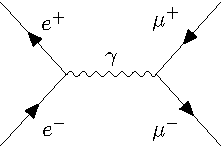
\includegraphics{etomu.pdf}
    \vspace{-30pt}
\end{figure}
\begin{align}
    \La_{QED} &= \bar{\psi}(i\cancel{\p}-m)\psi - \frac14F_{\mu\nu}F^{\mu\nu} - \frac{\alpha}{2}(\p_\mu A^\mu)^2 - eA^\mu j^\mu
\end{align}
The first term of this is the free spinor field, the second is the free electromagnetic field, the third is a gauge-fixing term with $\alpha=1$, and the fourth is the interaction term, with a current $j^\mu = \bar{\psi}\gamma^\mu\psi$.\\
\textit{If you're a physicist, we don't do social interactions, we just emulate them in whatever programming we run.}

\section{Feynman Rules}
What are the "building blocks"?
\begin{itemize}
    \item Terms with two fields give the propagators $\implies$ the Green's functions of the equations of motions
    \item Particles:
        \begin{figure}[H]
            \centering
            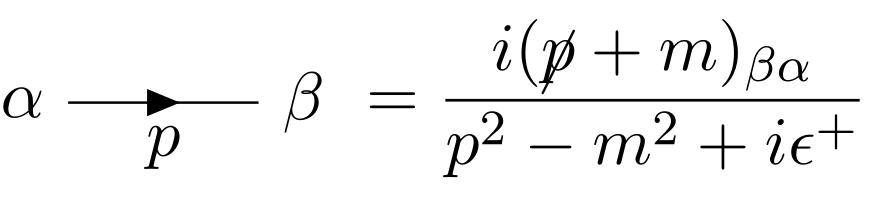
\includegraphics[scale=0.2]{feyn1.png}
        \end{figure}
    \item Propagators:
        \begin{figure}[H]
            \centering
            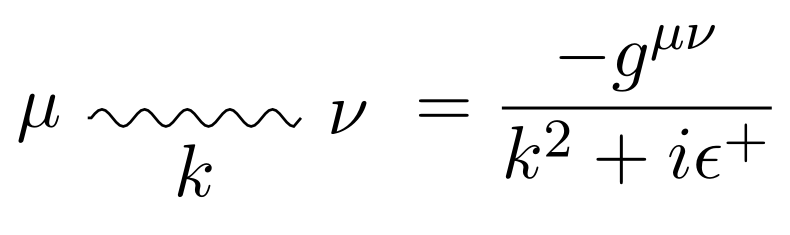
\includegraphics[scale=0.2]{feyn2.png}
        \end{figure}
    \item Vertices (interaction):
        \begin{figure}[H]
            \centering
            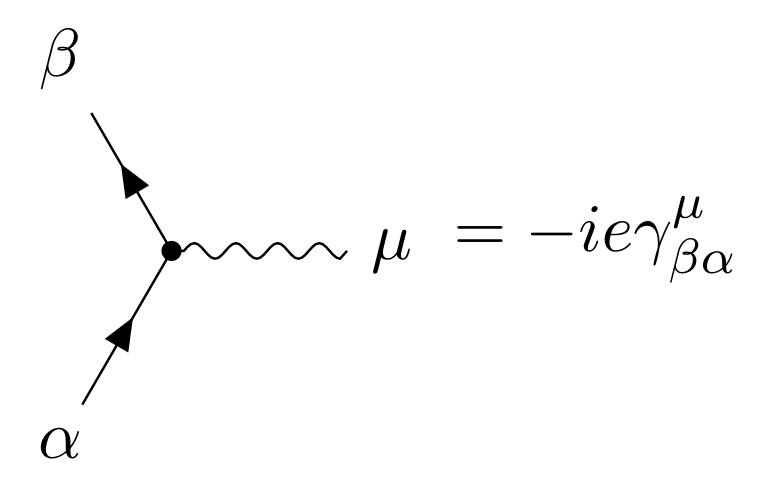
\includegraphics[scale=0.2]{feyn3.png}
        \end{figure}
\end{itemize}
Now the rules:
\begin{enumerate}
    \item Draw all distinct Feynman diagrams, including labels for the momenta of the incoming and outgoing particles:
        \begin{itemize}
            \item Incoming/outgoing (anti-)fermions with momentum $p$ are represented with spinors:\\ $u(p)/\bar{u}(p)$,  $(\bar{v}(p)/v(p))$
            \item Incoming/outgoing photons with momentum $k$ are represented with polarisation vectors $\e^\mu(k)$, /$\e^{*\mu}(k)$
            \item Propagators related to the external particles are "amputated"
        \end{itemize}
    \item Internal lines give rise to the corresponding propagators
    \item Interactions are represented by vertices and corresponding expression.
        We impose four momentum conservation at each vertex, thereby fixing the momenta of internal lines.
    \item $i$ (imaginary unit) times the amplitude related to a single diagram is given by the product of all building blocks, the single-diagram amplitudes are summed to yield the overall amplitude.
\end{enumerate}
\begin{figure}[H]
    \centering
    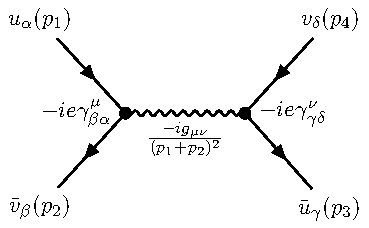
\includegraphics{etomu2.pdf}
    \vspace{-25pt}
\end{figure}
\begin{align}
    i\mathcal{M} &= \left[\bar{u}_{\alpha}(p_3)(-ie\gamma^\mu_{\alpha\beta})v_\beta(p_4)\right]\frac{-ig_{\mu\nu}}{(p_3+p_4)^2+i\e^+}\left[\bar{v}_\gamma(p_2)(-ie\gamma^\nu_{\gamma\delta}u_\delta(p_1)\right]
\end{align}
We now want to square this, so we sum over outgoing polarisations, average over incomings.
\begin{align}
    \frac14\sum_{spins}|\mathcal{M}|^2 &= -\frac{e^4}{4}\sum_{spins}\left[\bar{u}_\alpha(p_3)\gamma_{\alpha\beta}^\mu v_\beta(p_4)\bar{v}_{\beta'}(p_4)\gamma_{\beta'\alpha'}^{\mu'}u_{\alpha'}(p_3)\right]\frac{g_{\mu\nu}g_{\mu'\nu'}}{(p_3+p_4)^4}\left[\bar{v}_\gamma(p_2)\gamma^\nu_{\gamma\delta}u_\delta(p_1)\bar{u}_{\delta'}(p_1)\gamma^{\nu'}_{\delta'\gamma'}v_{\gamma'}(p_2)\right] \\
    \sum_{spin} &u_{\delta}(p)\bar{u}_{\delta'}(p) = (\cancel{p}-m)_{\delta\delta'},~ \sum_{spin} v_\beta\bar{v}_{\beta'} = (\cancel{p}+m)_{\beta\beta'} \\
    \frac14\sum_{spins}|\mathcal{M}|^2 &= \frac{e^4}{4}\text{Tr}\left[(\cancel{p}_3-m_3)\gamma^\mu(\cancel{p}_4+m_4)\gamma^\mu\right]\frac{g_{\mu\nu}g_{\mu'\nu'}}{(p_3+p_4)^4}\text{Tr}\left[(\cancel{p}_2+m_2)\gamma^\nu(\cancel{p}_1-m_1)\gamma^{\nu'}\right] \\
    \text{Tr}[\gamma^\mu\gamma^\nu] &= 4g^{\mu\nu},~ \text{Tr}[\gamma^\mu\gamma^\nu\gamma^\rho\gamma^\sigma] = 4(g^{\mu\nu}g^{\rho\sigma}+g^{\mu\sigma}g^{\nu\rho}-g^{\mu\rho}g^{\nu\sigma}) \\
    \frac14\sum_{spins}|\mathcal{M}|^2&=\text{Tr}[pp\gamma^\rho\gamma^\mu\gamma^\delta\gamma^{\mu'}]-\text{Tr}[m_3m_4\gamma^\mu\gamma^{\mu'}] \\
                                      &= 4p_{4\delta}p_{3\rho}\left(\gamma^{\rho\mu}g^{\delta\mu'}-g^{\rho\delta}g^{\mu\mu'}+g^{\rho\mu'}g^{\mu\delta}\right) - 4m_3m_4g^{\mu\mu'} \\
                                      &= \left[4(p_4^\mu p_3^{\mu'}+ p_4^{\mu'}p_3^\mu - g^{\mu\mu'}p_3p_4)-4m_\mu^2g^{\mu\mu'}\right]\times\left[4(p_2^\nu p_1^{\nu'}+p_2^{\nu'}p_1^\nu - g^{\nu\nu'}p_1p_2)-4m_e^2g^{\nu\nu'}\right],\; m_i = 0 \\
                                      &= \frac{16e^4}{4(p_3+p_4)^4}\left[2(p_2p_4)(p_1p_3) + 2(p_1p_4)(p_2p_3) - 4(p_1p_2)(p_3p_4) + 4(p_1p_2)(p_3p_4)\right] \\
                                      &= \frac{8e^4}{(p_3+p_4)^2}\left[(p_2p_4)(p_1p_3)+(p_1p_4)(p_2p_3)\right]
\end{align}

%\subfile{gauge.tex}
%\subfile{phenom.tex}
\end{document}
